\setchapterpreamble[u]{\margintoc}
\chapter{Summary of published results}
\label{ch:summary}
 
\begin{figure*}[htbp]
    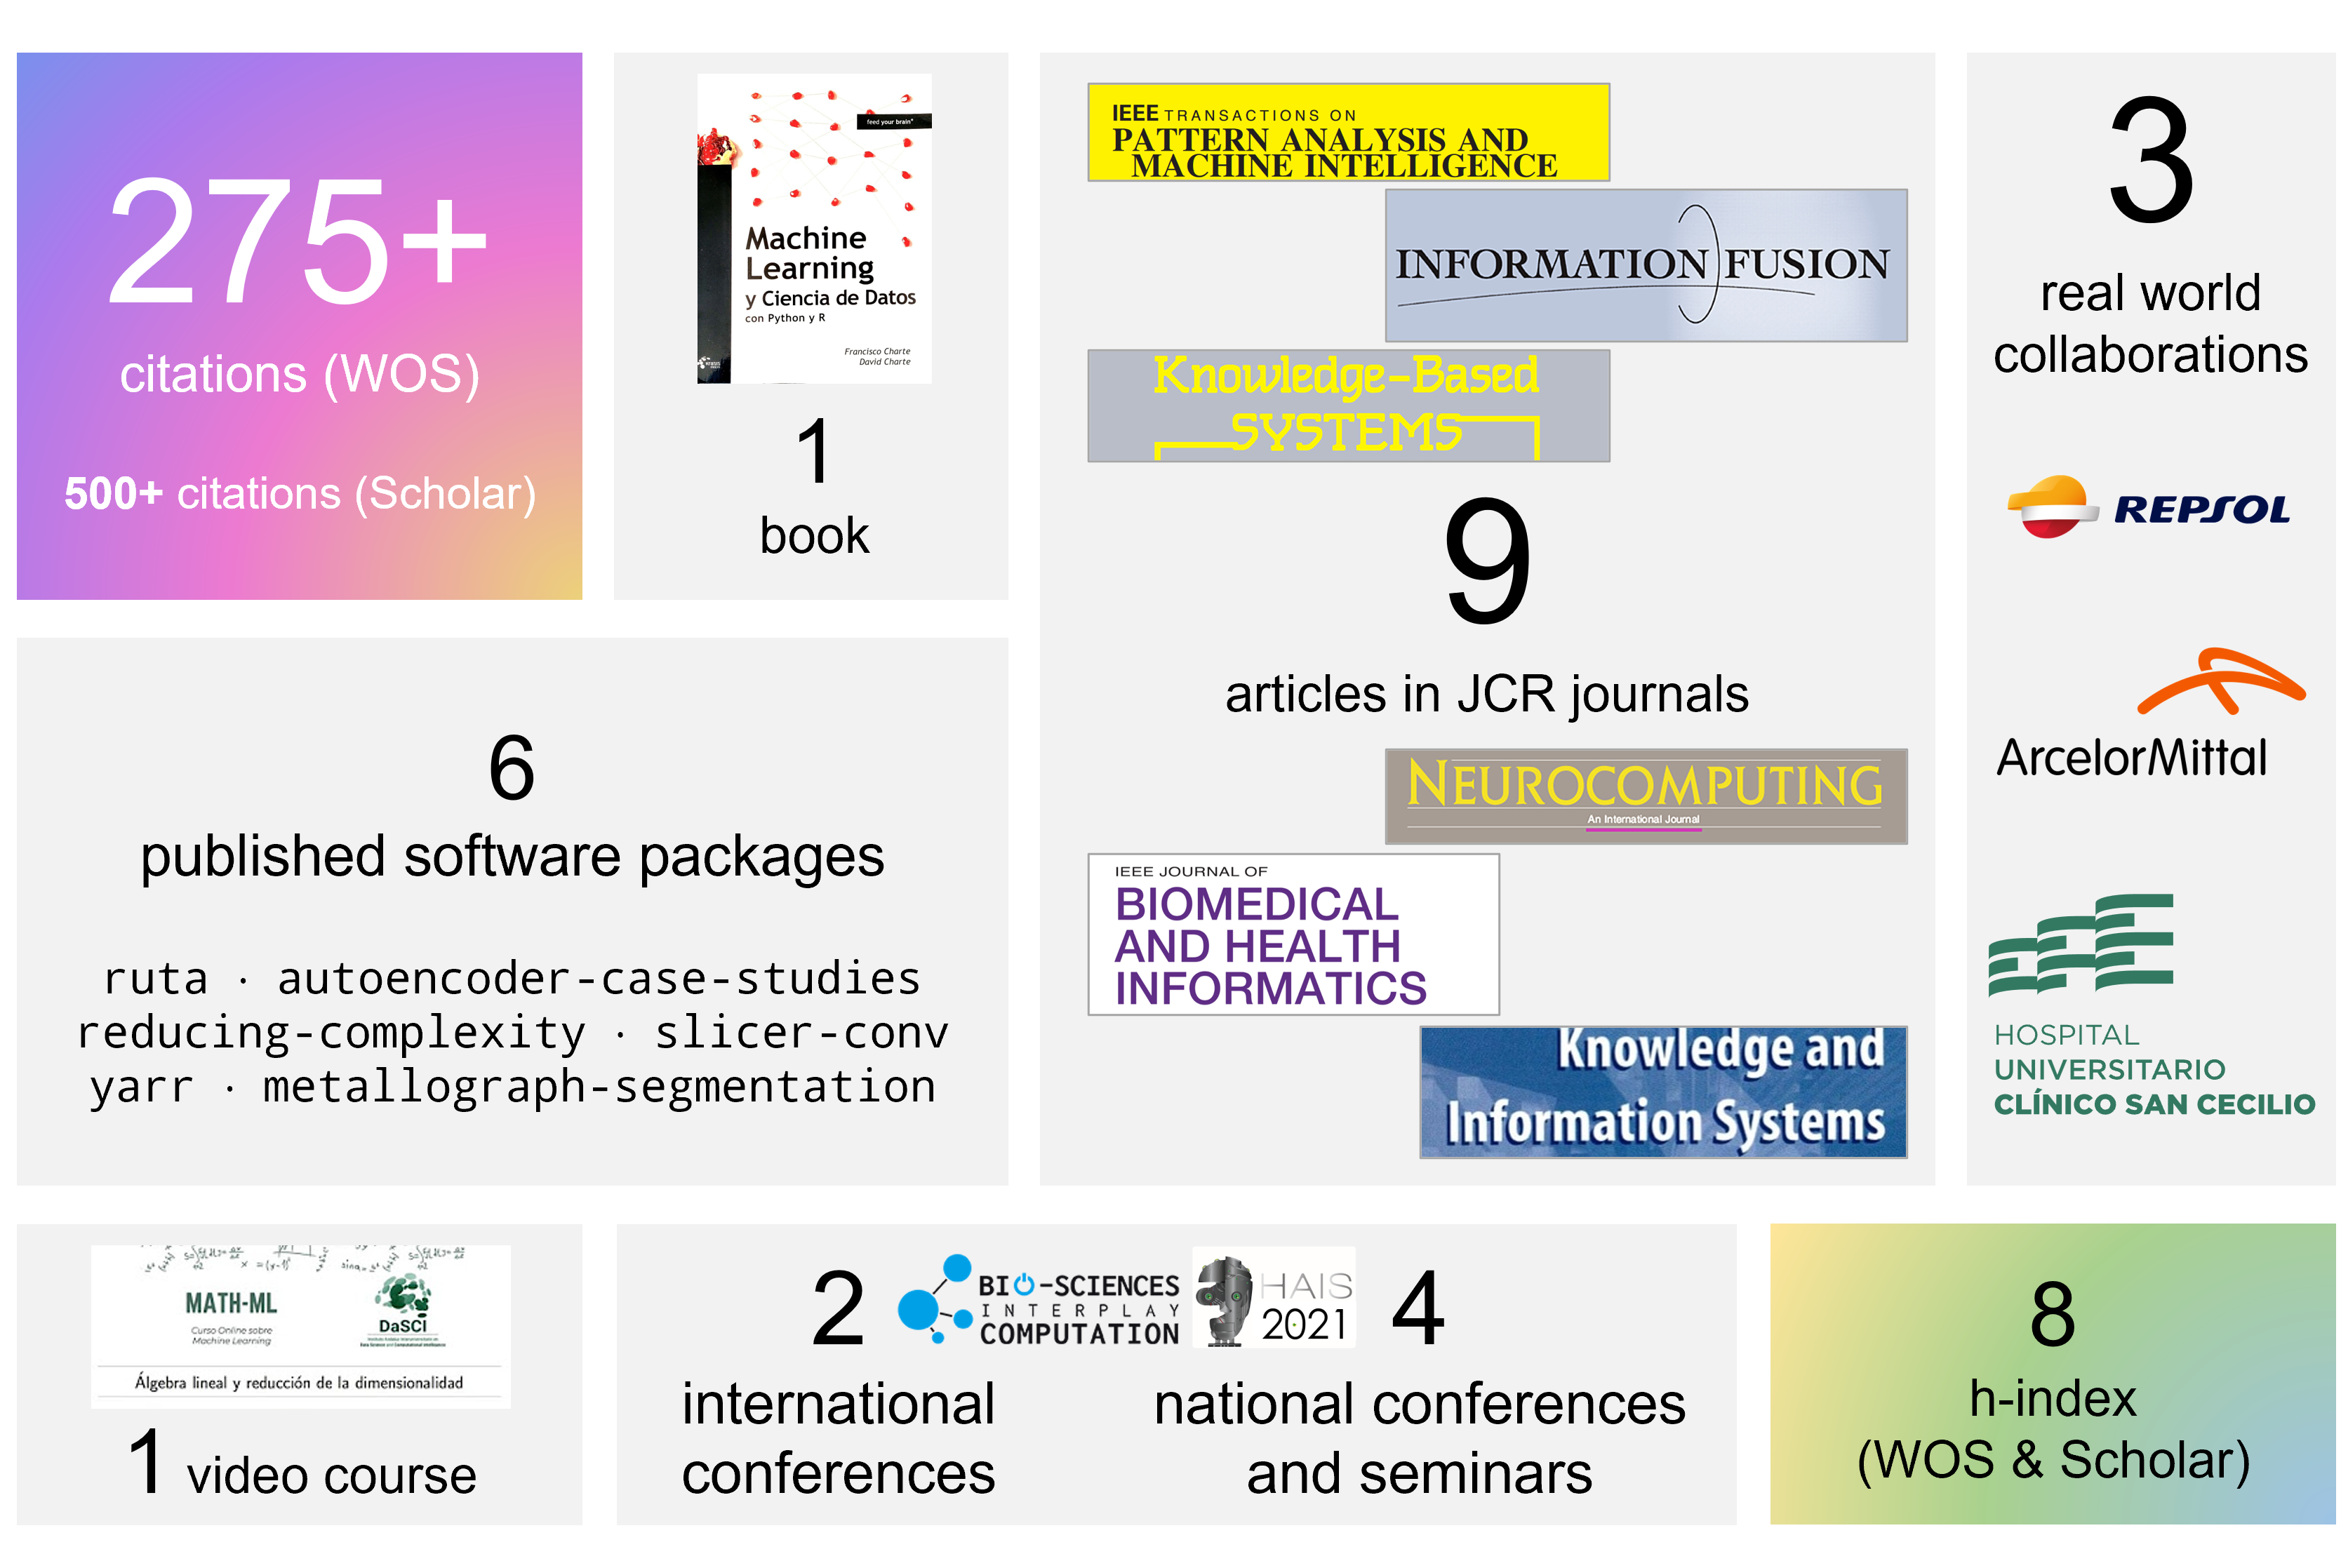
\includegraphics[width=\linewidth]{dashboard}
    \caption{\label{fig:dashboard}Visual summary of the main results obtained throughout the doctorate.}
\end{figure*}

\begin{figure*}
    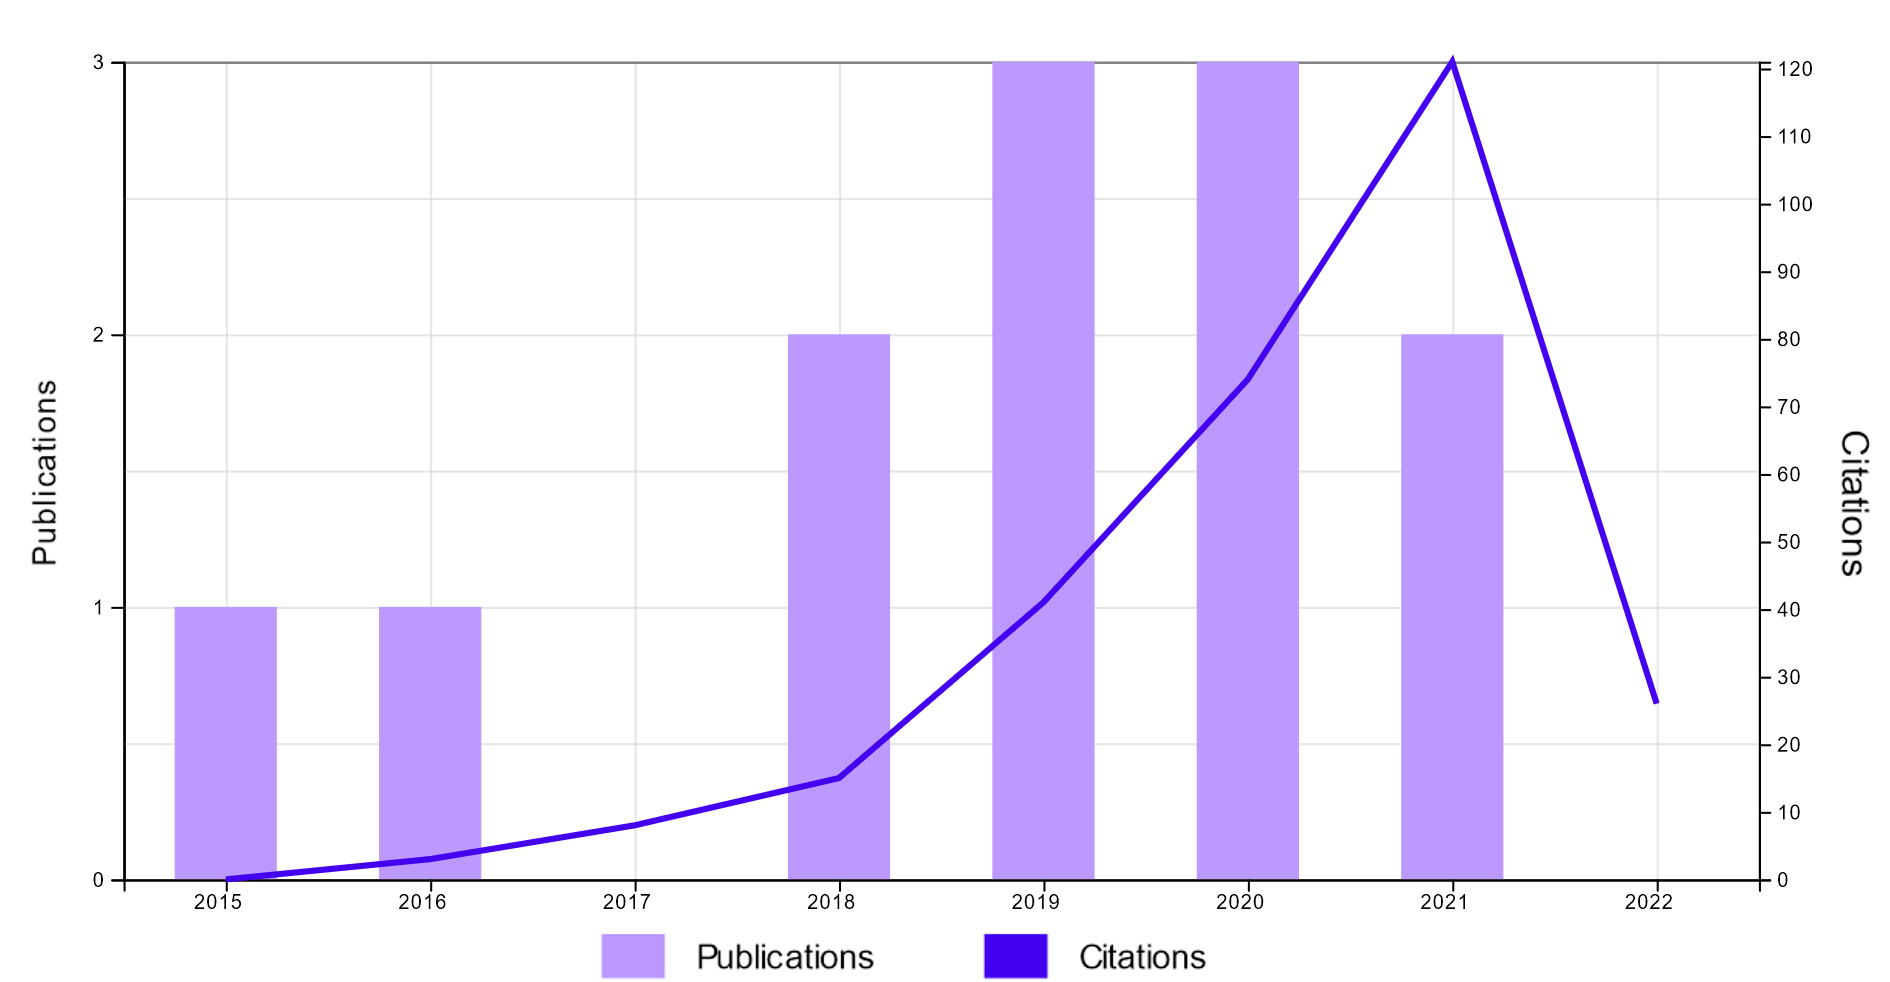
\includegraphics[width=\linewidth]{pubs}
    \caption{\label{fig:citations}Graph of the number of publications and citations across years (source: Web of Science).}
\end{figure*}

\begin{table*}
    \begin{tabular}[htbp]{lrrrr}
        \toprule
        Journal & IF & Q (JIF) & Q (JCI) & Category \\
        \midrule
        Pattern Analysis and Machine Intelligence
        & 16.389 & Q1 & Q1 & CS AI \\
        Information Fusion
        & 12.975 & Q1 & Q1 & CS AI \\
        Knowledge-Based Systems
        &  8.038 & Q1 & Q1 & CS AI \\
        Neurocomputing
        &  5.719 & Q1 & Q1 & CS AI \\
        Progress in Artificial Intelligence
        & - & - & Q4 & CS AI \\
        \midrule
        Knowledge and Information Systems 
        &  2.822 & Q2 & Q2 & CS AI, CS IS \\
        Biomedical and Health Informatics
        &  5.772 & Q1 & Q1 & CS IS \\
        \bottomrule
    \end{tabular}
    \caption{\label{tbl:journals}Quality metrics of the journals where articles have been coauthored by the candidate during the course of the thesis. Columns indicate the impact factor (IF) and the quartile according to Journal Impact Factor (JIF) and Journal Citation Indicator (JCI).}
\end{table*}